\section{Empirical Results}
\label{sec:bleuresult}

In this section, we present the empirical results to prove our hypothesis that \textit{BLEU is not effective in evaluating translation quality of source code migration task}
\subsection{Correlation between BLEU and Semantic scores}
Regarding the first part of the hypothesis (the use of BLEU for a single model), we show the relation
between BLEU scores and human judgments via semantic scores. We use
Pearson's correlation coefficient~\cite{PearsonCorrelation} to gauge
how strong their relation is. The correlation coefficient has value
between -1 and 1, where 1 indicates the strongest positive relation, -1
indicates the strongest negative relation, and 0 indicates no relation at
all.

Figures~\ref{fig:BleuSemlpSMT} and~\ref{fig:BleuSemMppSMT} show the
scatter plots between two metrics: BLEU and Semantic. Each point
represents the scores of a pair of methods where its $x$-axis value is
for BLEU scores and $y$-axis value is for Semantic scores. The
correlation coefficient between BLEU and Semantic scores for the model
mppSMT is 0.523 and for the model lpSMT is 0.570. That meant there is a
positive relationship between the two metrics, but it is weak
since the correlation is closer to 0.5 than to 1.0. The two
Figures~\ref{fig:BleuSemlpSMT} and~\ref{fig:BleuSemMppSMT} also
demonstrate the weak correlation due to the following observations:

\emph{Observation 1:} For a fixed value of Semantic score, there can
be many associated BLEU values. Specifically, in the model lpSMT, with
a Semantic Score of 1, the BLEU scores can vary greatly between 0-1,
which is reflected on the top horizontal line of dots in the
Figure~\ref{fig:BleuSemlpSMT}. Similarly, in
Figure~\ref{fig:BleuSemMppSMT}, with the Semantic Score of 1, the BLEU
scores are in the range of 0.5 to 1.

From this observation, it can be implied that translated code can have
low BLEU score, but high Semantic score. This can be explained by two
reasons. First, a translated method can use different code structure
to perform the same functionality. For example, the translated method
that got maximum Semantic score (a raw score is 4, normalized score is
1) on Figure~\ref{fig:scoreEG} has low BLEU score (0.4) because it
uses a \code{for} loop instead of a \code{foreach} loop as in the
reference code. Second, there is also the whitespace issue. For
example, the translated method has the tokens \code{m()}, but the
reference method has \code{m ()}. The former is interpreted as one
token while the former is interpreted as two tokens. This situation
reduces the precision on phrases, but the human subject still
evaluated the result with high Semantic score.

\emph{Observation 2:} For a fixed value of BLEU, there can be many
associated Semantic scores. For instance,
Figure~\ref{fig:BleuSemMppSMT} shows that for a high BLEU score, a
value around 0.75 can have Semantic Score from 0.25 to 1. This can be
observed by the vertical line of dots in the figure.

From this observation, it can be implied that a translated method can
have high BLEU score, but low Semantic score. There are two reasons
for this. The first reason is that if a translated method has multiple
correct phrases, but in the incorrect order, the method can still be
useless and justified as so in human judgment.
%
For example, in Figure~\ref{fig:issueexample2}, the translated method
misplaces the position of the bracelet which makes the method has low
Semantic score, but high BLEU score. Another reason for this
implication is that resulting method does not capture the important
program elements. For example, the result contains mostly keywords and
punctuation such as \code{if}, \code{public}, \code{()}, but misses
out the important program elements such as function calls or variable
names. In this case, it will have low Semantic score while having
a moderate to high BLEU score.

In conclusion, BLEU does not reflect well the
semantics of source code, and it is not suitable to use in evaluating
semantic accuracy of a SMT-based code migration system.

\subsection{The Use of BLEU in Comparing Models}
To validate the use of BLEU in comparing different SMT-based code migration systems, we conduct study to see if the change in BLEU scores over models reflect the change in translation quality represented by human judgments of Semantic score. For a same set of 375 original Java methods, the two models GNMT and mppSMT generates two sets of 375 translated methods. Each set has its own BLEU scores and Semantic scores. We ignored pairs of translated results if they have the same BLEU score or Semantic score (136 of the cases). For the remaining results, we found out that in \textbf{34\%} of the cases, the change in BLEU score contradicts the change in Semantic score. It means an improvement in BLEU score leads to a decrease in Semantic score and vice versa. In other words, if one function is translated by two migration models, one-third of the time, the result which has higher BLEU score actually has lower translation quality than the other. Consequently, BLEU is not reliable to use in comparing different SMT-based migration models. 

\begin{figure}
\caption{BLEU metric vs Semantic metric (lpSMT model)}
\centering
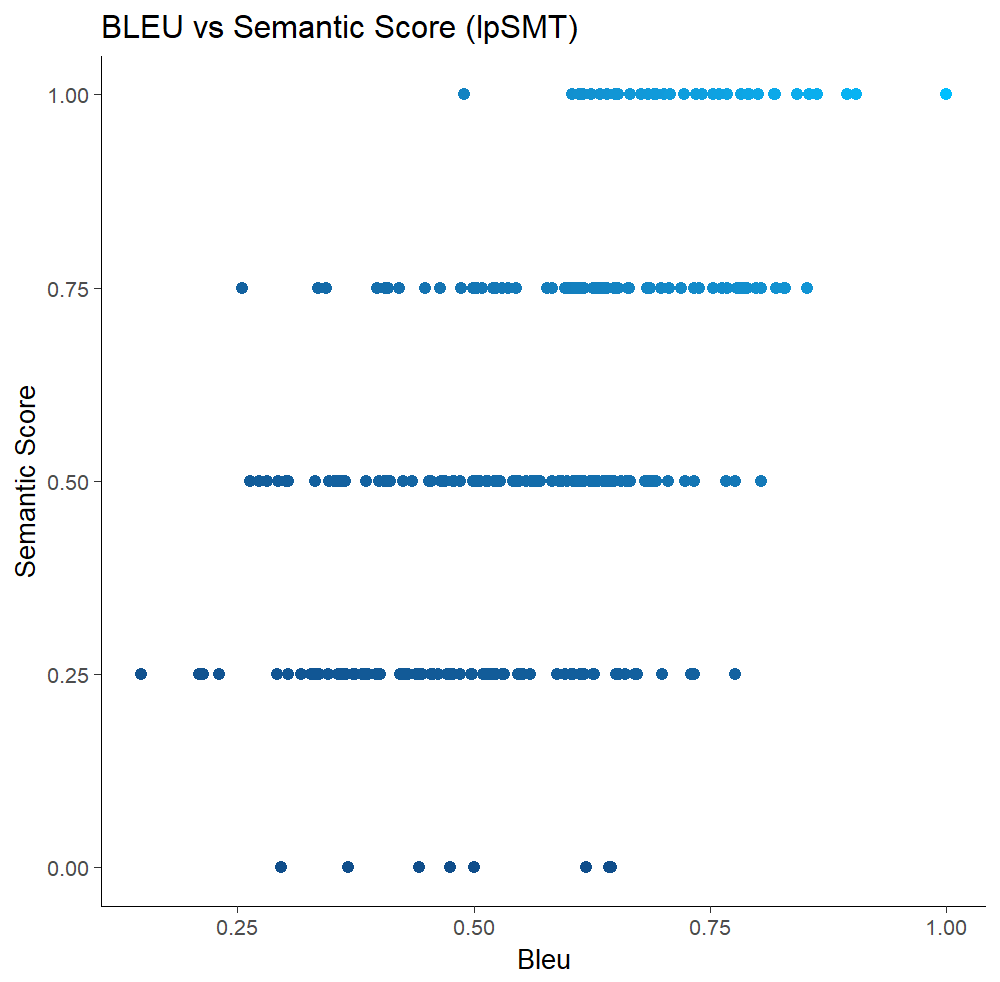
\includegraphics{img/bleuvssemantic_lpSMT.png}
\label{fig:BleuSemlpSMT}
\end{figure}

\begin{figure}
\caption{BLEU metric vs Semantic metric (mppSMT model)}
\centering
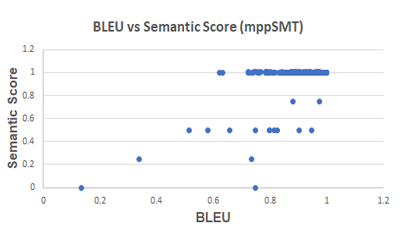
\includegraphics{img/bleuvssemantic_mppSMT.png}
\label{fig:BleuSemMppSMT}
\end{figure}

